\chapter{Sana System}
Sana System is believed to be an Iranian malware targeting Iranian cellphones. The virus logs the victim's phone number and sends it to a remote server. In addition, the virus also reads every incoming SMS message and forwards them to the aforementioned server: this could be used to steal sensitive information like 2FA codes. 
After doing some online research we discovered an article\footnote{\url{https://partonews.ir/en/from-the-fraud-of-3000-malware-the-loss-of-several-thousand-people-with-the-fake-sana-system-fata-police-seeing-a-judicial-notification-is-not-money/}} were it is mentioned that a similar virus with the same app name is installed from a fake minister of justice site where the user also inserts his bank account information under the pretext of showing juridical documents and, after infecting the user phone, sends malicious links to other phone contacts to spread the virus. We are certain that these viruses are different since the one we analyzed does not have any permission to access contacts info and write messages, however, it is important to highlight the stunning similarities in both presentation and SMS handling, as this could be an indication of them being part of the same phishing campaign originating from the same group.

\section{VirusTotal}
We started by feeding the APK to the VirusTotal tool:
\begin{figure}[H]
\centering
    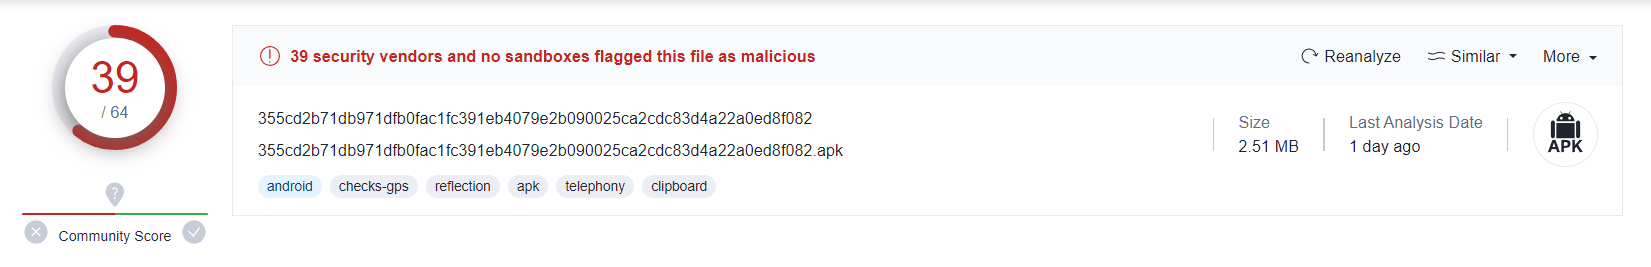
\includegraphics[width=1\textwidth]{./images/screenshot/SanaSystem/ReviewSanaSystem.png}
    \caption{Review score of Sana System}
    \label{fig:SanaReview}
\end{figure}

As it can be seen, the score of 39 out of 64 shows a very high chance of it being a virus. In general, many of the most popular anti-malware tools, like Avast or Kaspersky, correctly flag this software as malicious, as it can be seen in Fig. \ref{fig:SanaDetection}.

\begin{figure}[h!]
\centering
    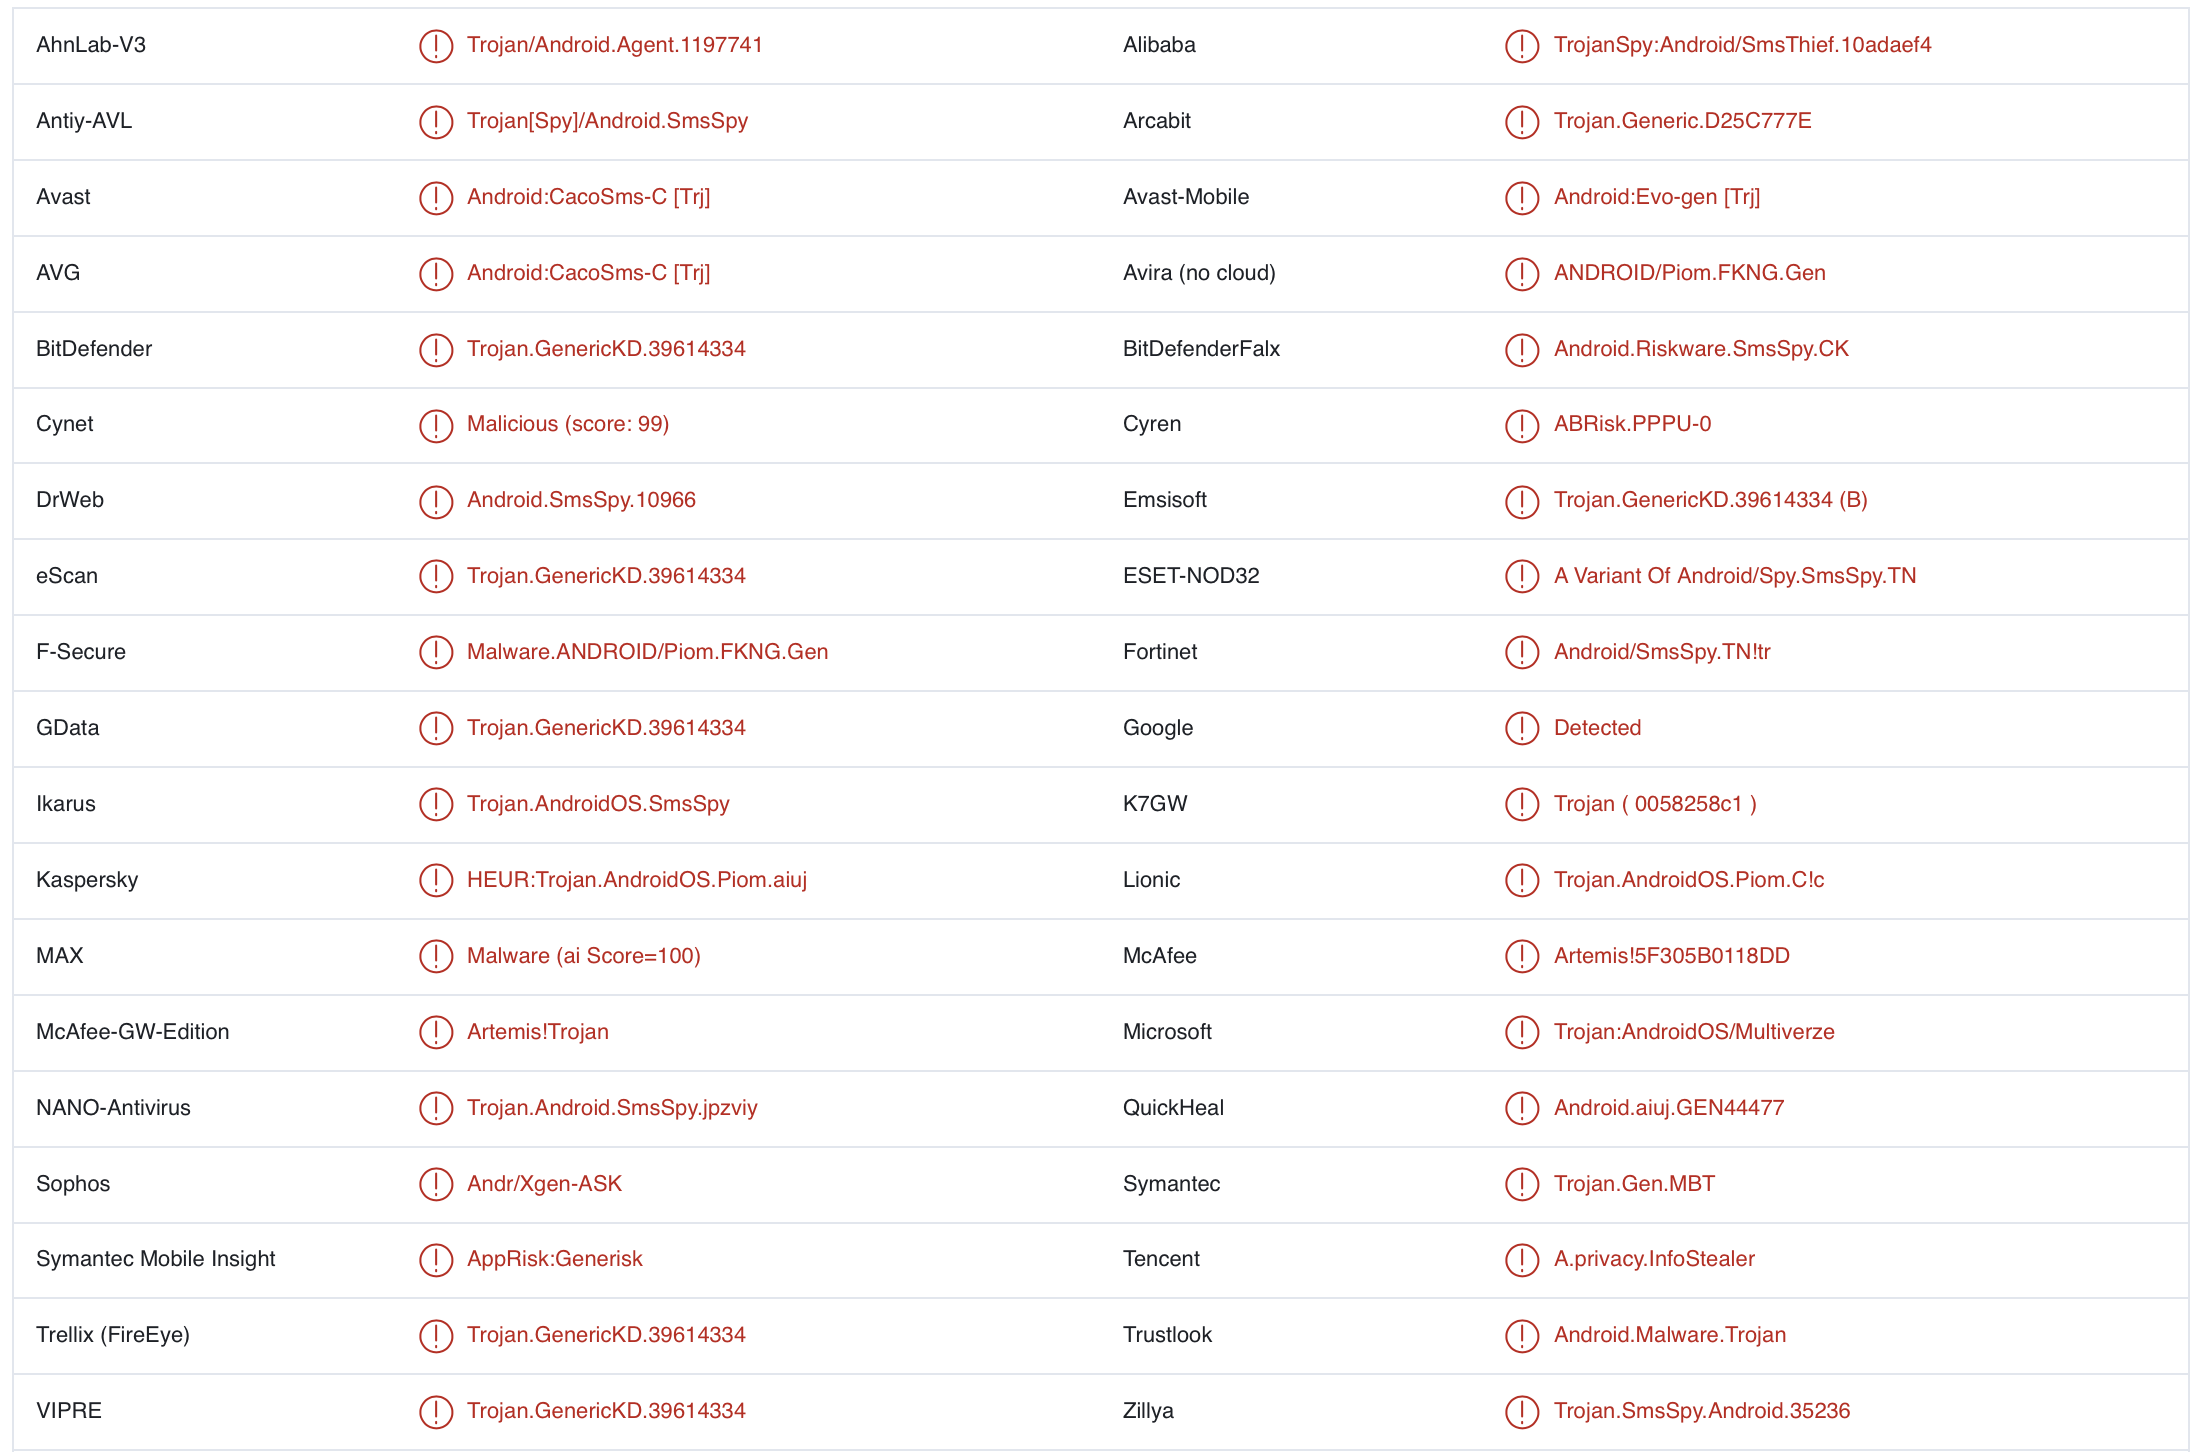
\includegraphics[width=1\textwidth]{./images/screenshot/SanaSystem/Detection.png}
    \caption{Anti-malware detection}
    \label{fig:SanaDetection}
\end{figure}

In general, the malware is identified as a trojan/smsspy: this is also indicated by the permissions required by the app.
\begin{figure}
\centering
    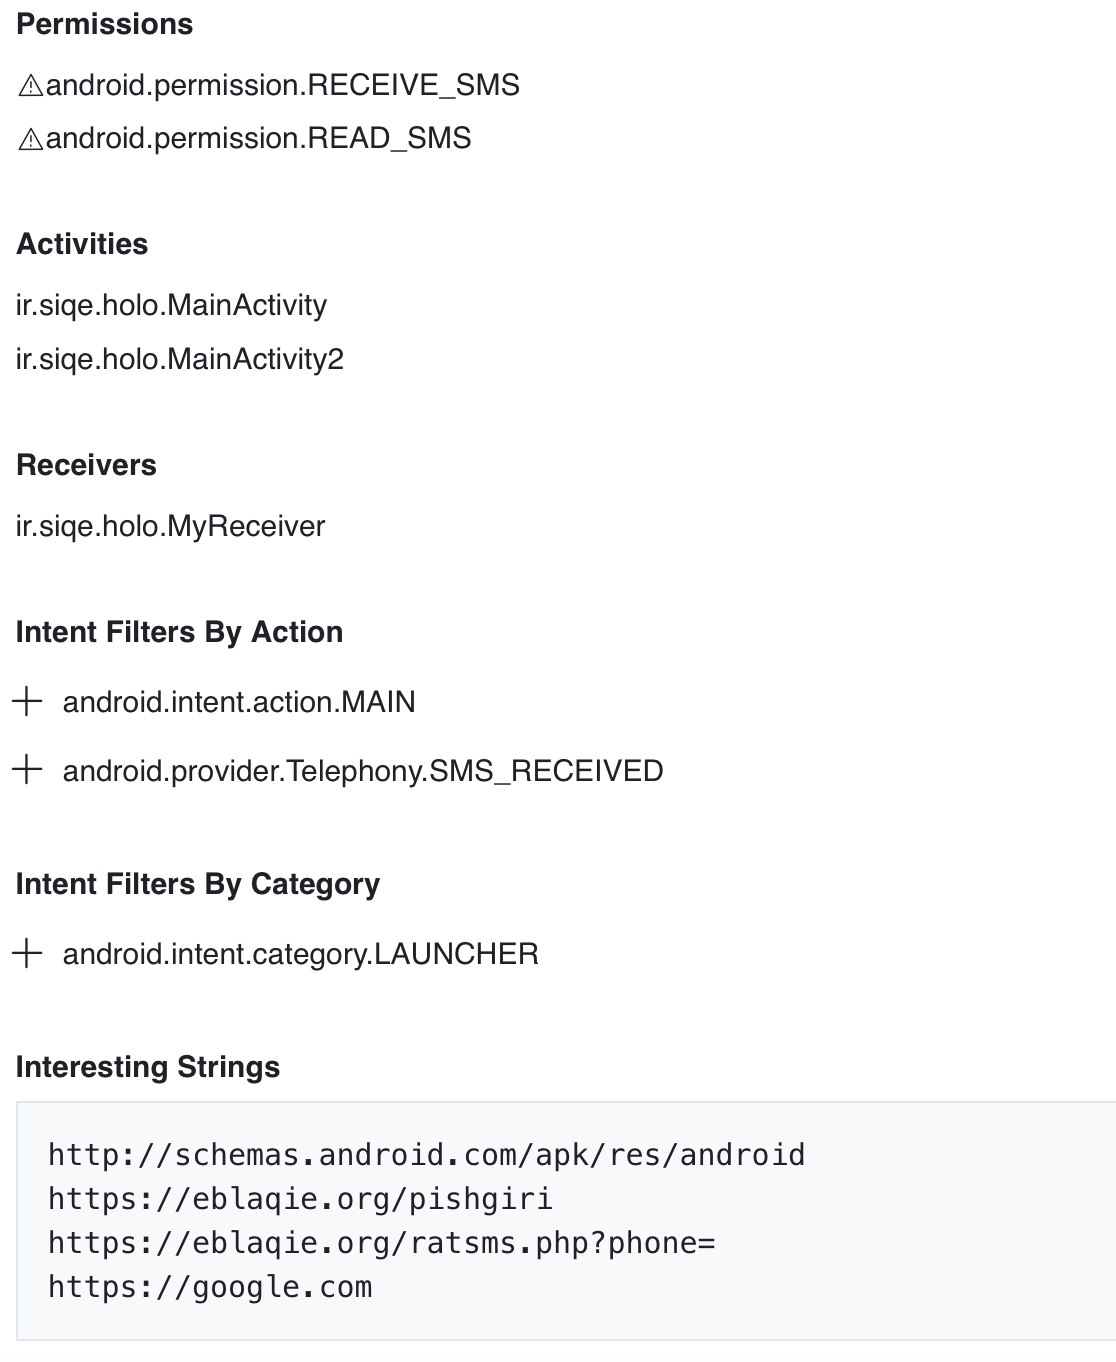
\includegraphics[scale=0.5]{./images/screenshot/SanaSystem/Details.png}
    \caption{Details highlighted by virus total}
    \label{fig:SanaDetails}
\end{figure}
As shown in Fig. \ref{fig:SanaDetails} the app requests permission to receive SMS messages and read them. In addition, it requires permission to access the network state and establish internet connections. This can be seen in the manifest Fig \ref{fig:SanaManifest}.
\begin{figure}[h!]
\centering
    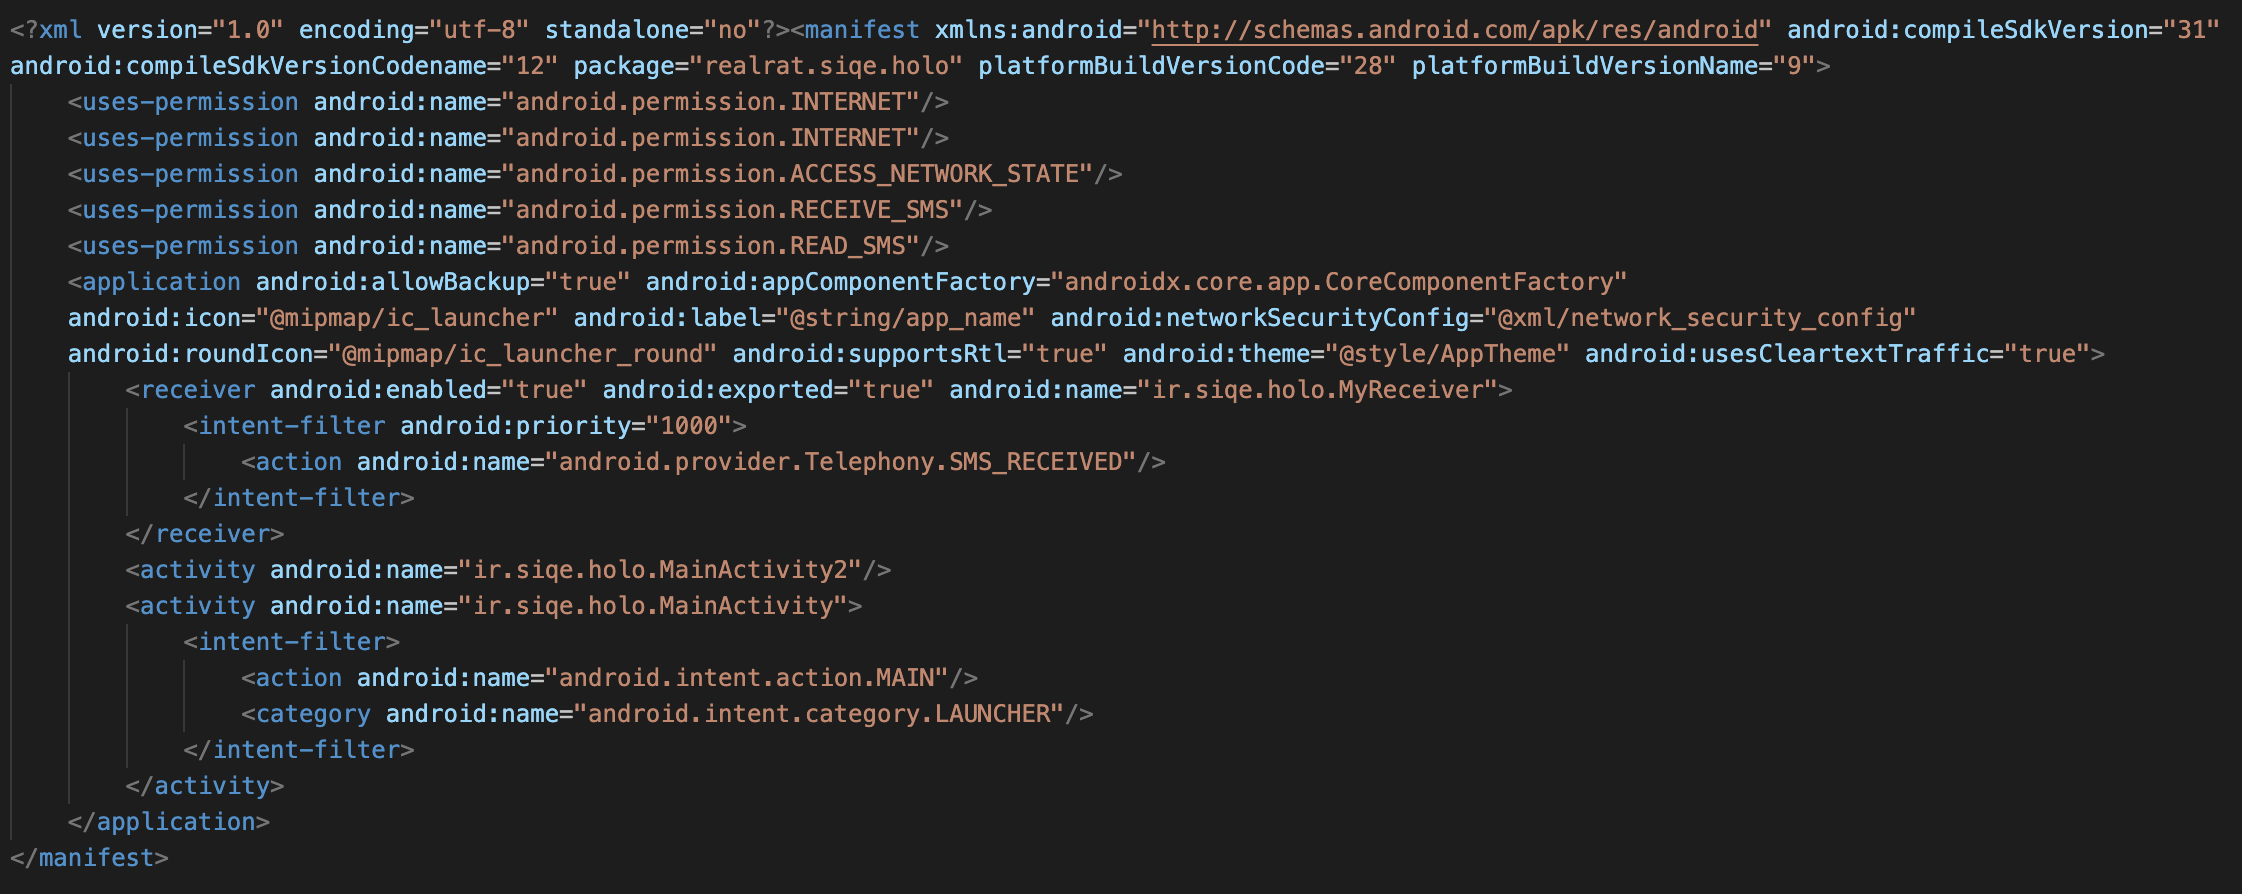
\includegraphics[width=1\textwidth]{./images/screenshot/SanaSystem/Manifest.png}
    \caption{App manifest}
    \label{fig:SanaManifest}
\end{figure}

Virus total also signaled the presence of some interesting string such as: \\
"\texttt{https://eblaqie.org/pishgiri}" and "\texttt{//eblaqie.org/ratsms.php?phone=}". In particular the second one, as we shall see in the next pages, is used to perform a GET operation to a server where the phone number and relative SMS messages are logged.

In addition Virus Total shows us the detected contacted domains, where \texttt{eblaqie.org} is present and is the only one reached by the app Fig. \ref{fig:ContactedDom}.
\begin{figure}
\centering
    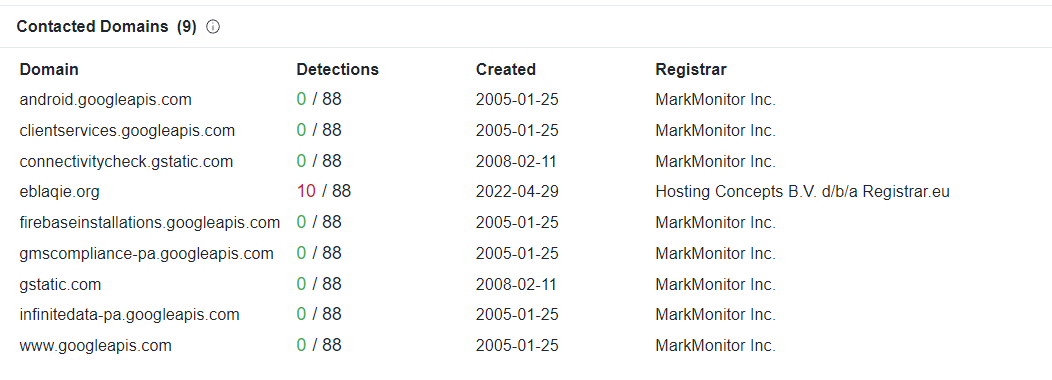
\includegraphics[width=1\textwidth]{./images/screenshot/SanaSystem/Domains.png}
    \caption{Contacted domains}
    \label{fig:ContactedDom}
\end{figure}


\section{MobSF}
We then proceed by feeding the APK to MobSF and got the header in Fig. \ref{fig:mobsfHeader}. Due to the exhaustiveness of Virus Total's report, we decided not to show the almost identical results of the static analysis. 

\begin{figure}[h!]
\centering
    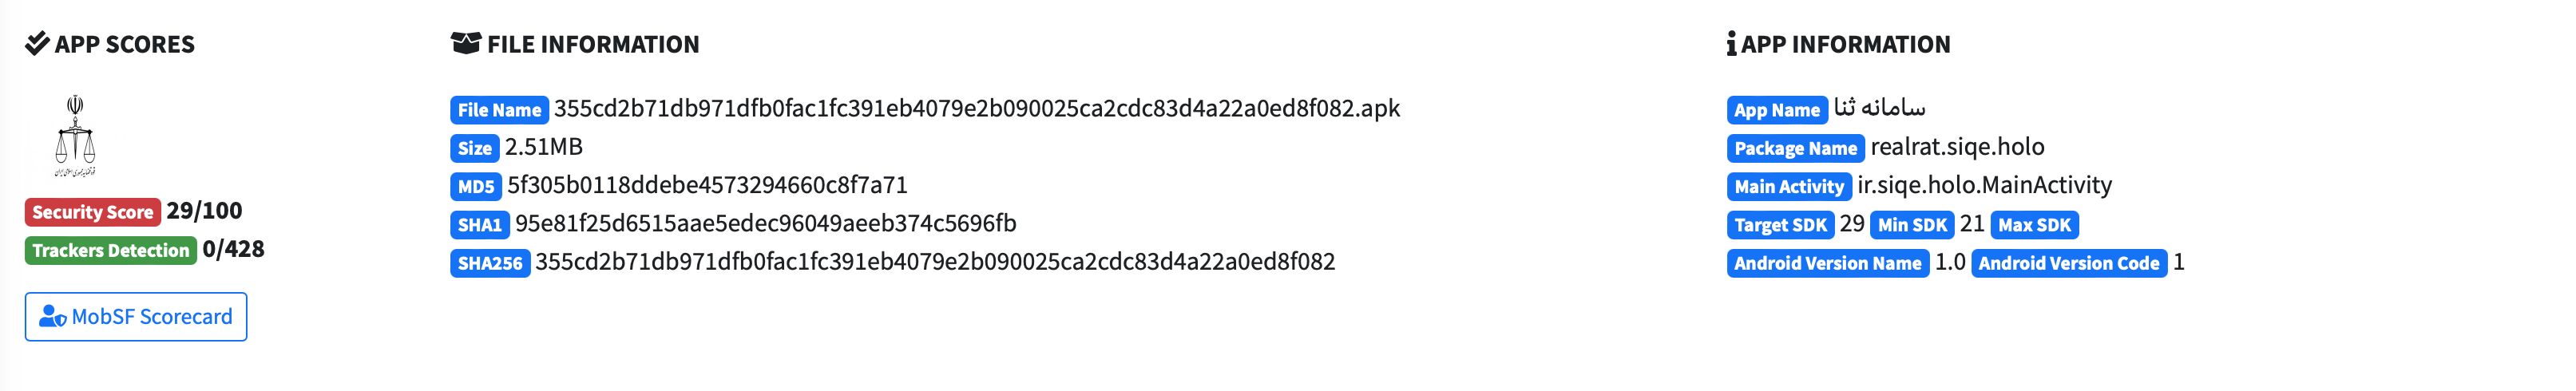
\includegraphics[width=1\textwidth]{./images/screenshot/SanaSystem/HeaderMobSF.png}
    \caption{Header of MobSF}
    \label{fig:mobsfHeader}
\end{figure}

Another thing to point out is that \texttt{eblaqie.org} is signaled by Maltrail \footnote{\url{https://github.com/stamparm/maltrail}}, using a publicly available domain blacklist, as a malicious domain and is therefore not to be trusted (Fig. \ref{fig:MalTrail}). 

\begin{figure}[h!]
\centering
    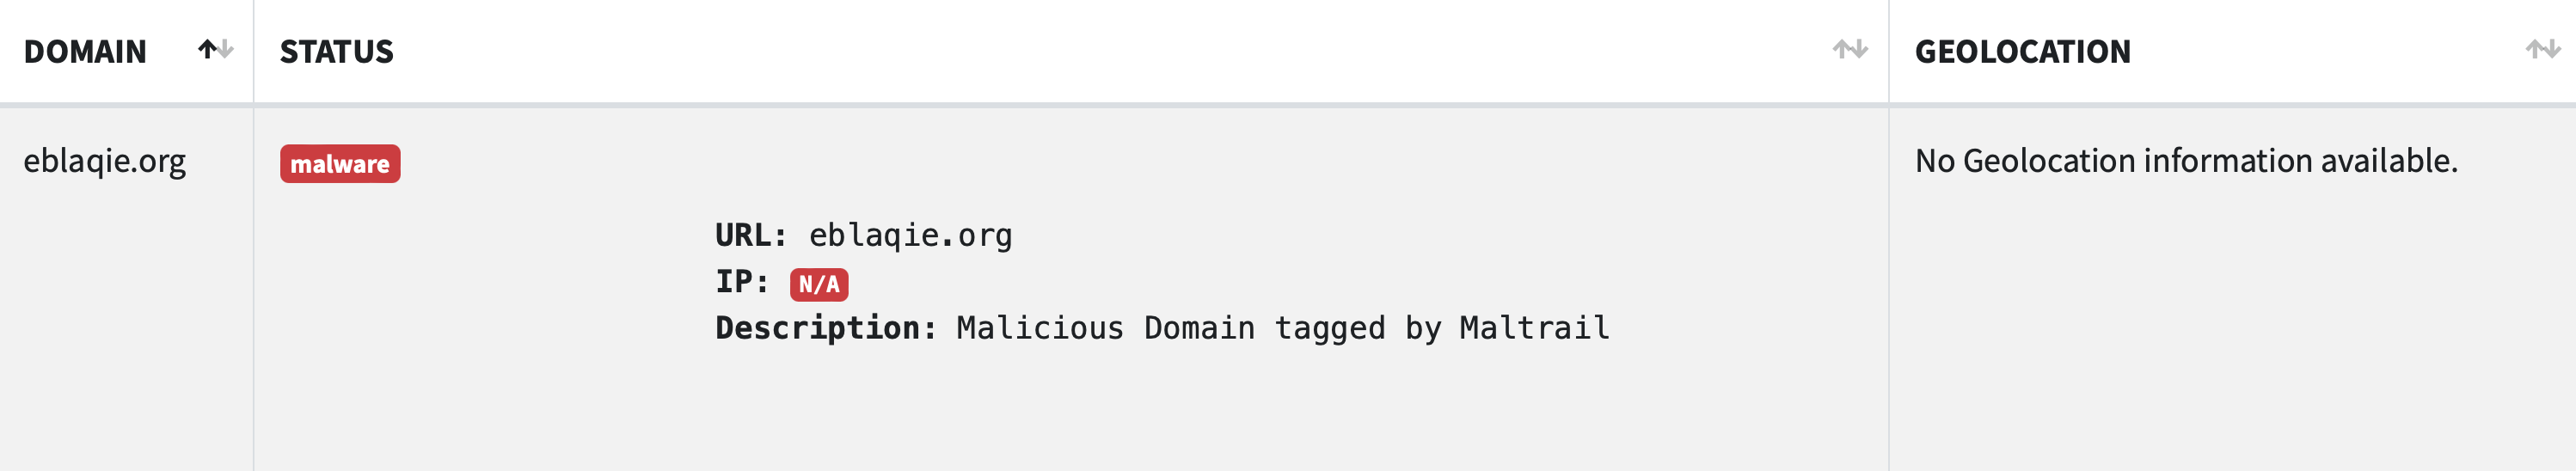
\includegraphics[width=1\textwidth]{./images/screenshot/SanaSystem/eblaqieDomain.png}
    \caption{Tag of eblaqie.org}
    \label{fig:MalTrail}
\end{figure}

\section{Code Analysis}
We start this code analysis by looking into the code structure shown in Fig. \ref{fig:SanaPackage} and specifically into \texttt{ir.siqe.holo} package highlighted by MobSF in Fig. \ref{fig:mobsfHeader} where the main activity is placed. Virus total (Fig. \ref{fig:SanaDetails}) also confirms \texttt{MainActivity} to be the entry point of the software. The other packages are public libraries and there is no evidence of them being tampered with.

\begin{figure}[h!]
\centering
    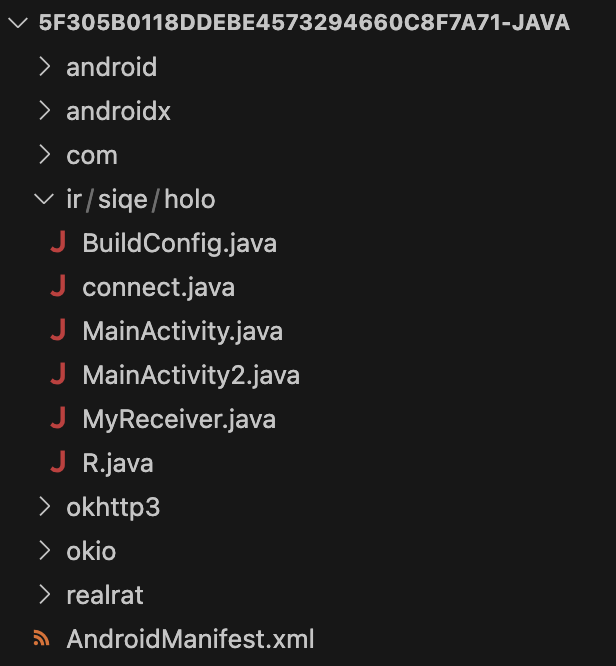
\includegraphics[width=0.6\textwidth]{./images/screenshot/SanaSystem/Package.png}
    \caption{Package organization}
    \label{fig:SanaPackage}
\end{figure}
\newpage

\subsection{MainActivity}
\texttt{MainActivity} (Fig.\ref{fig:MainActivity}) extends \texttt{AppCompatActivity} which allows to use newer features of android on older devices and, given the fact that the minimum SDK required to run the software is Android 5.0, allows the use of this app on devices that have no longer received security updates. After the activity is launched, the \texttt{onCreate} method is called. \texttt{Bundle} is typically used for passing data between various Android activities. After setting the screen presented to the user, the app waits for a text input in the form of a number. Then when the user clicks on the button with id "\textit{go}" there is a check with a regular expression, for matching an iranian telephone number (+98 as prefix), if the number doesn't match, it displays a small popup (Toast) that says \textit{"The mobile number is not valid"} and does nothing else, otherwise asks for permission to read SMS messages and, if granted, calls the method \texttt{connect} to log to a remote server the inputted number with a string identifying the new entry, then a new activity starts and the code stream goes to \texttt{MainActivity2}.

\begin{figure}[h!]
\centering
    \includegraphics[width=1\textwidth]{./images/screenshot/SanaSystem/MainActivity.png}
    \caption{MainActivity}
    \label{fig:MainActivity}
\end{figure}

\subsection{connect}
The constructor of the \texttt{connect} class in Fig. \ref{fig:Connect} takes as input two strings: the first is reserved for the mobile phone number, the second is reserved for additional information, like \textit{"Installed new target"} in \texttt{MainActivity}, or the content of the intercepted SMS, and the third is the context, used for information about an application environment. The method initializes the context of \texttt{AndroidNetworking}, that is a third party library built on top of \texttt{okHtpp} (\url{https://square.github.io/okhttp/}), which is present on the package. Then the app performs a GET request to \texttt{https://eblaqie.org/ratsms.php} where the phone number and an info string containing for example the text of received sms are passed, in case of a correct response the app does nothing, otherwise try to send the same info to google probably for debugging purposes. We do not know what the server does with the phone number and info received however given the nature of the info field, we hypothesize the server logs the information for stealing sensitive information, like 2FA codes.

\begin{figure}[h!]
\centering
    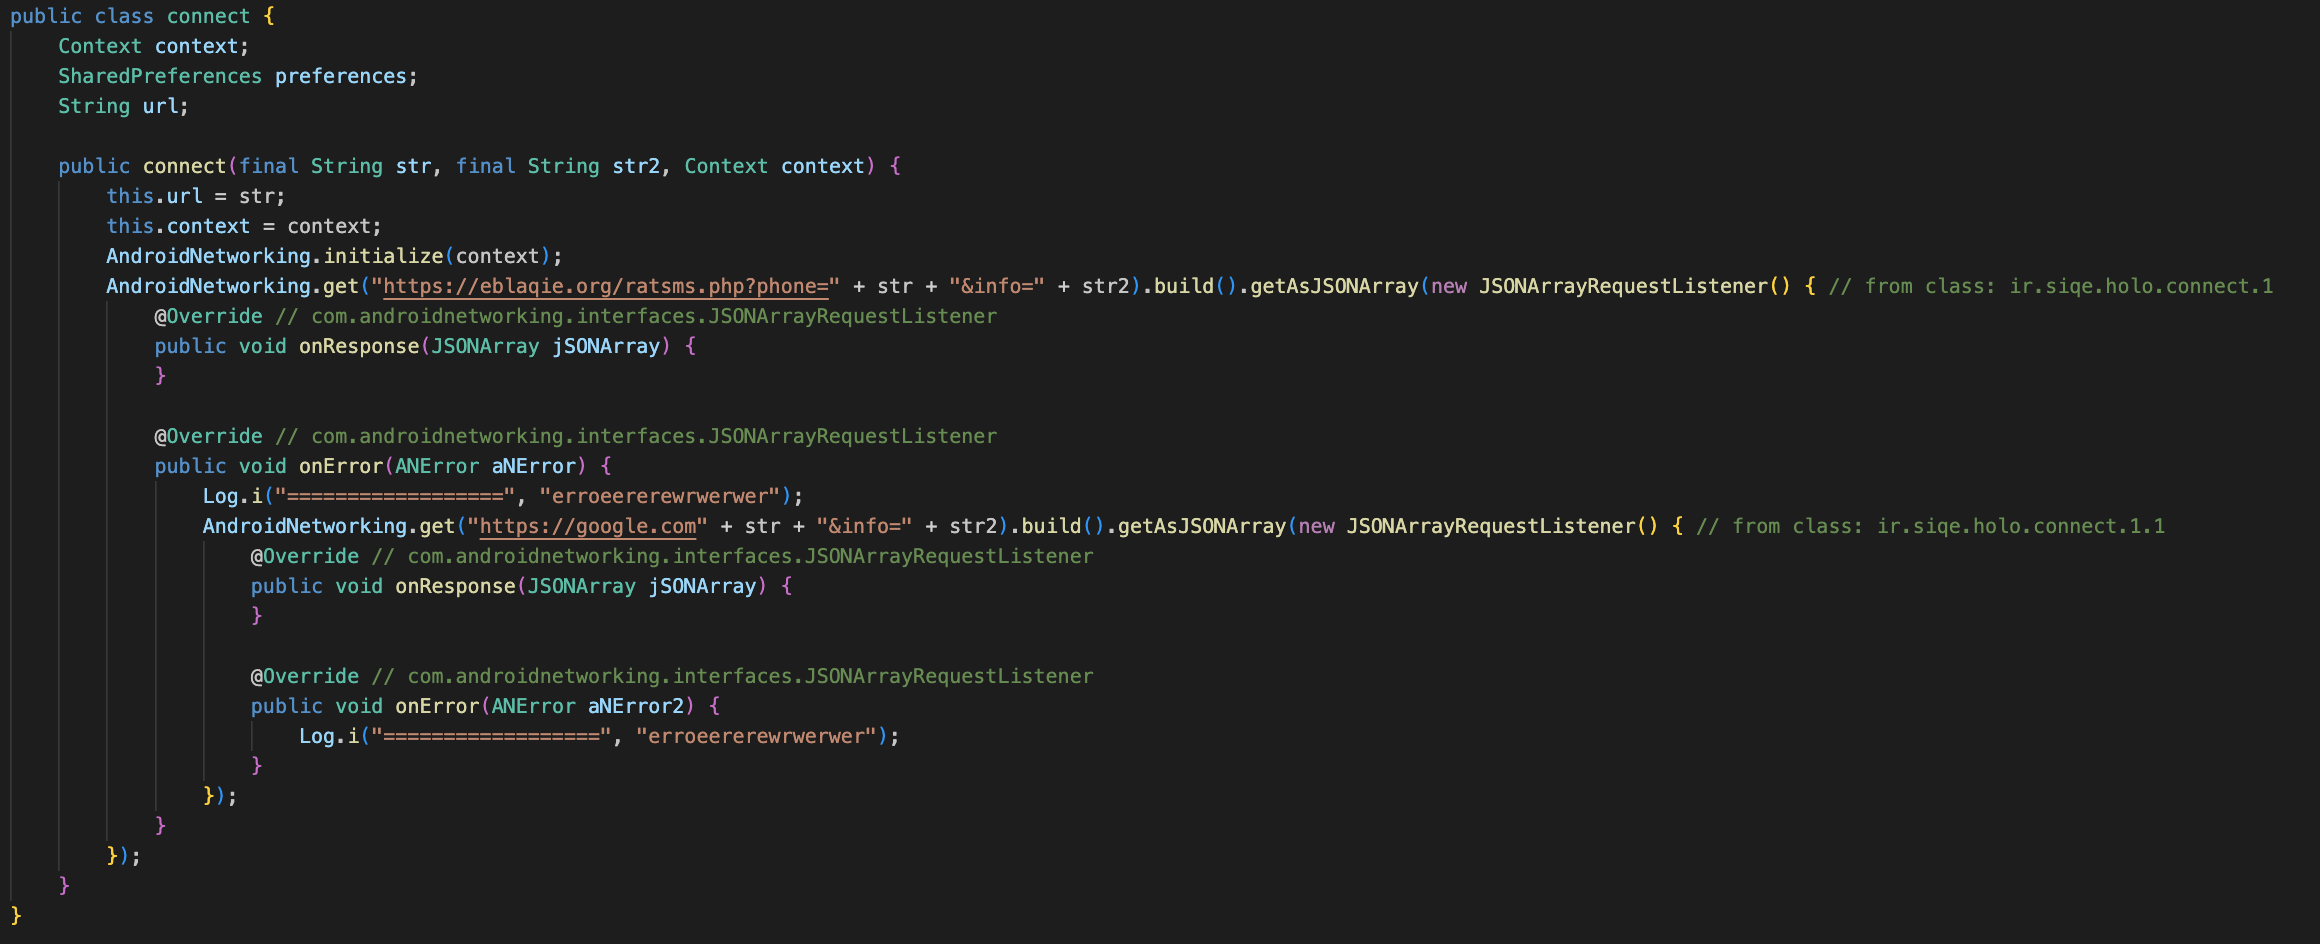
\includegraphics[width=1\textwidth]{./images/screenshot/SanaSystem/connect.png}
    \caption{Connect}
    \label{fig:Connect}
\end{figure}

\subsection{MainActivity2}
The \texttt{MainActivity2} (Fig.\ref{fig:MainActivity2}) code sets up a \texttt{WebView} for the following url: \url{https://eblaqie.org/pishgiri}. There are other methods for error handling, that only record logs, and there's a custom back navigation, that only displays "back to exit" but does nothing. It is important to notice that \texttt{pishgiri.org} is a legit site so there is the possibility for the app to load a fake site for banking application, however the fake url has been taken down so it is no longer possible to confirm that.

\begin{figure}[h!]
\centering
    \includegraphics[width=1\textwidth]{./images/screenshot/SanaSystem/MainActivity2.png}
    \caption{MainActivity2}
    \label{fig:MainActivity2}
\end{figure}

\subsection{myReceiver}
Finally \texttt{myReceiver} (Fig.\ref{fig:myReceiver}) extends \texttt{BroadcastReceiver} which allows the class to inherit methods called when a broadcast message is received, like an SMS. After the phase of message handling in the form of PDUs, which send binary information in 7 bit or 8 bit format, where the messages are concatenated in a single string, if the string contains the persian word for "night site" the sharedPreferences are updated, otherwise the line terminator is replaced with a space " " and the logging operation to the remote server is performed.
\begin{figure}[h!]
\centering
    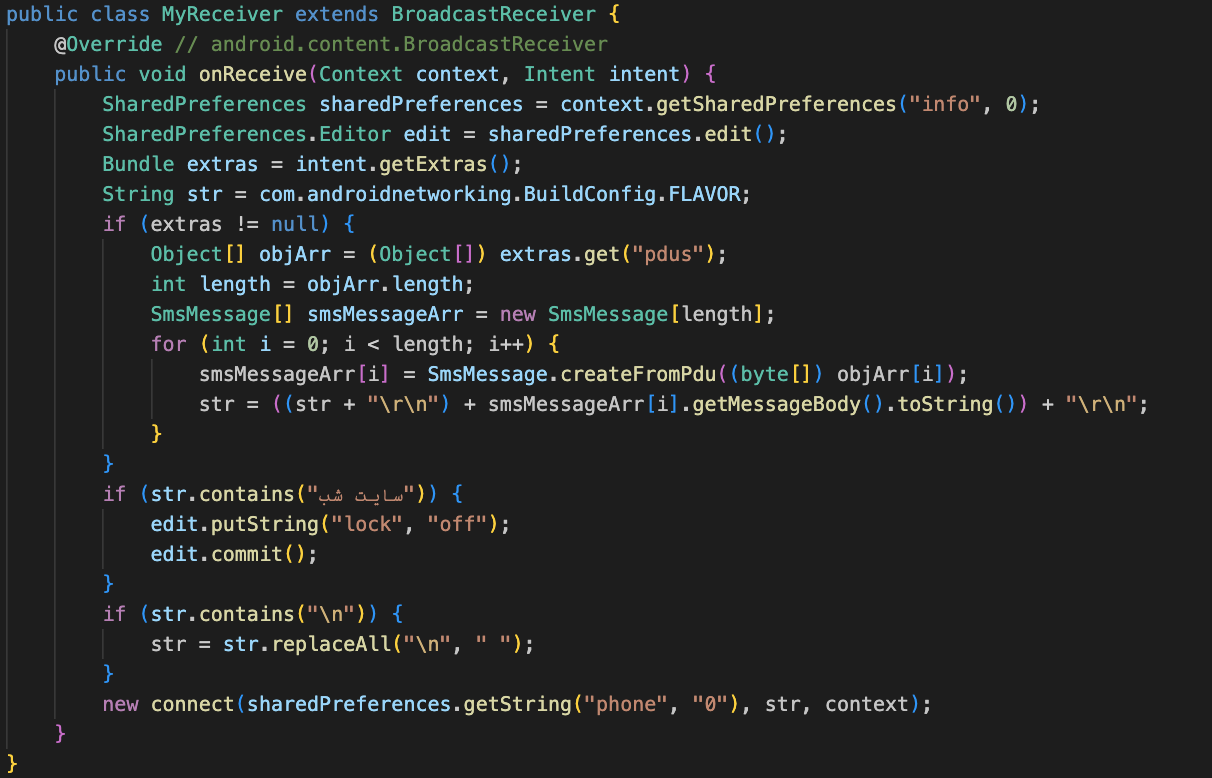
\includegraphics[width=1\textwidth]{./images/screenshot/SanaSystem/myReceiver.png}
    \caption{myReceiver}
    \label{fig:myReceiver}
\end{figure}

As a final comment on the virus, there is a high chance for this virus to lead to a fake banking site were usernames and passwords are stolen and then the 2FA code is also stolen through the logging of SMS messages. However, as said before, due to the malicious site being taken down, we cannot confirm our hypothesis.

\section{Dynamic analysis}
\label{sec:sana-sys-dyn-anal}
To better understand the actual behavior of the virus and confirm what has been discovered during the static analysis, we performed a dynamic analysis of the malware in a safe and isolated virtual environment.
Using an Android Virtual Device from the Android Studio development environment (\url{https://developer.android.com/studio}), we were able to emulate a Google Pixel 2 phone with Android API 30 (Android 11) running inside QEMU.
\begin{figure}[h!]
\centering
    
\includegraphics[width=1\textwidth]{./images/screenshot/SanaSystem/dynamic_and_proxy/icon.png}
    \caption{Sana System application icon}
    \label{fig:sana-system-icon}
\end{figure}
Once installed, the application presents itself as per Fig. \ref{fig:sana-system-icon}

\begin{figure}[h!]
	\begin{subfigure}[h]{0.32\textwidth}
	    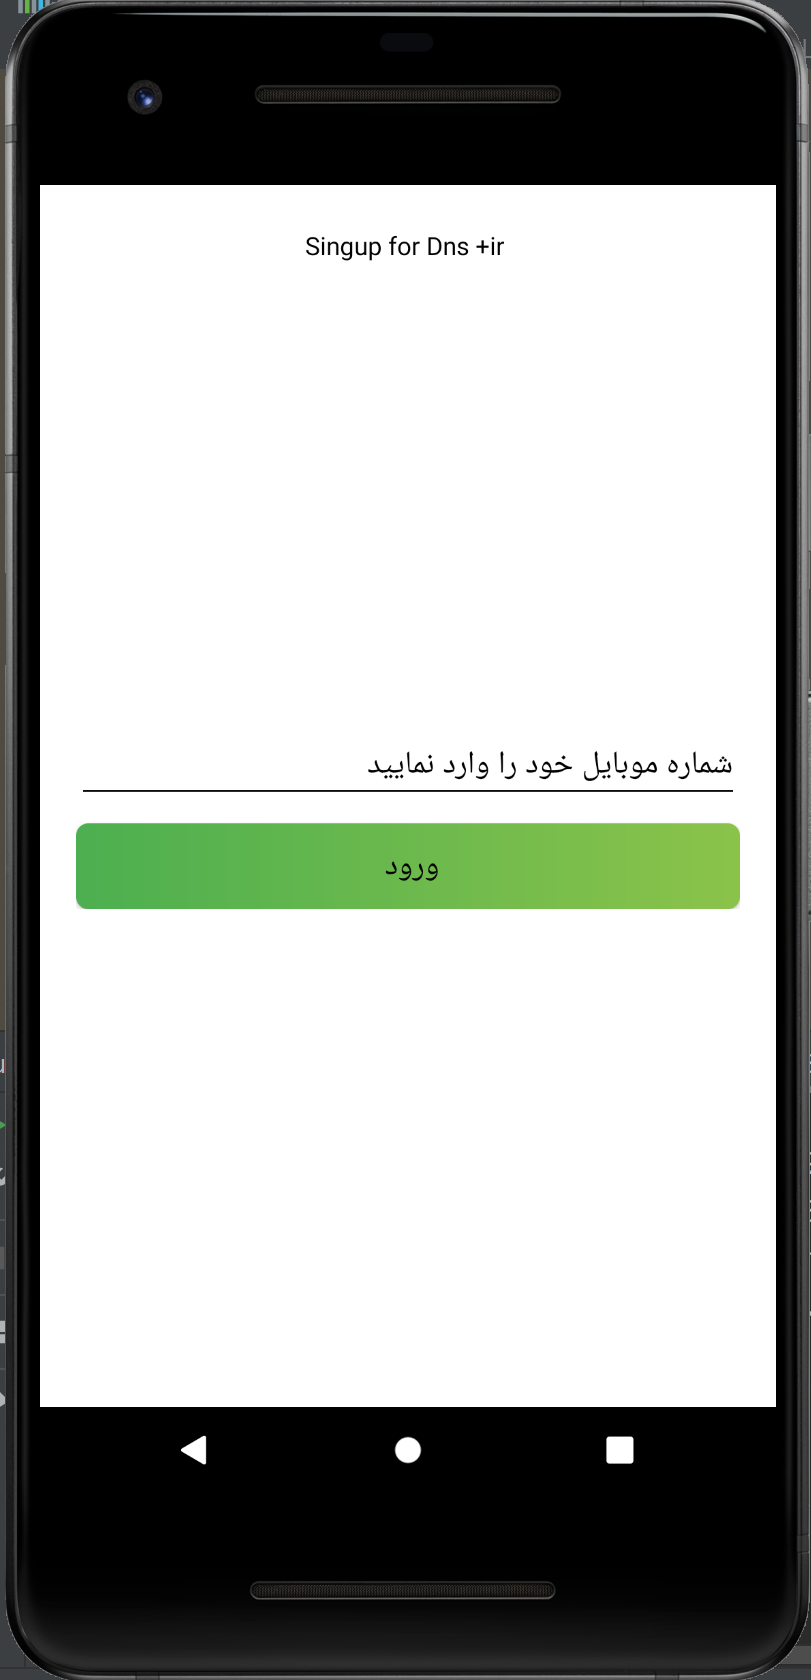
\includegraphics[width=1\textwidth]{./images/screenshot/SanaSystem/dynamic_and_proxy/main_page.png}
	    \caption{Sana System application main page}
	    \label{fig:sana-system-main-page}
    \end{subfigure}
    \begin{subfigure}[h]{0.32\textwidth}
	    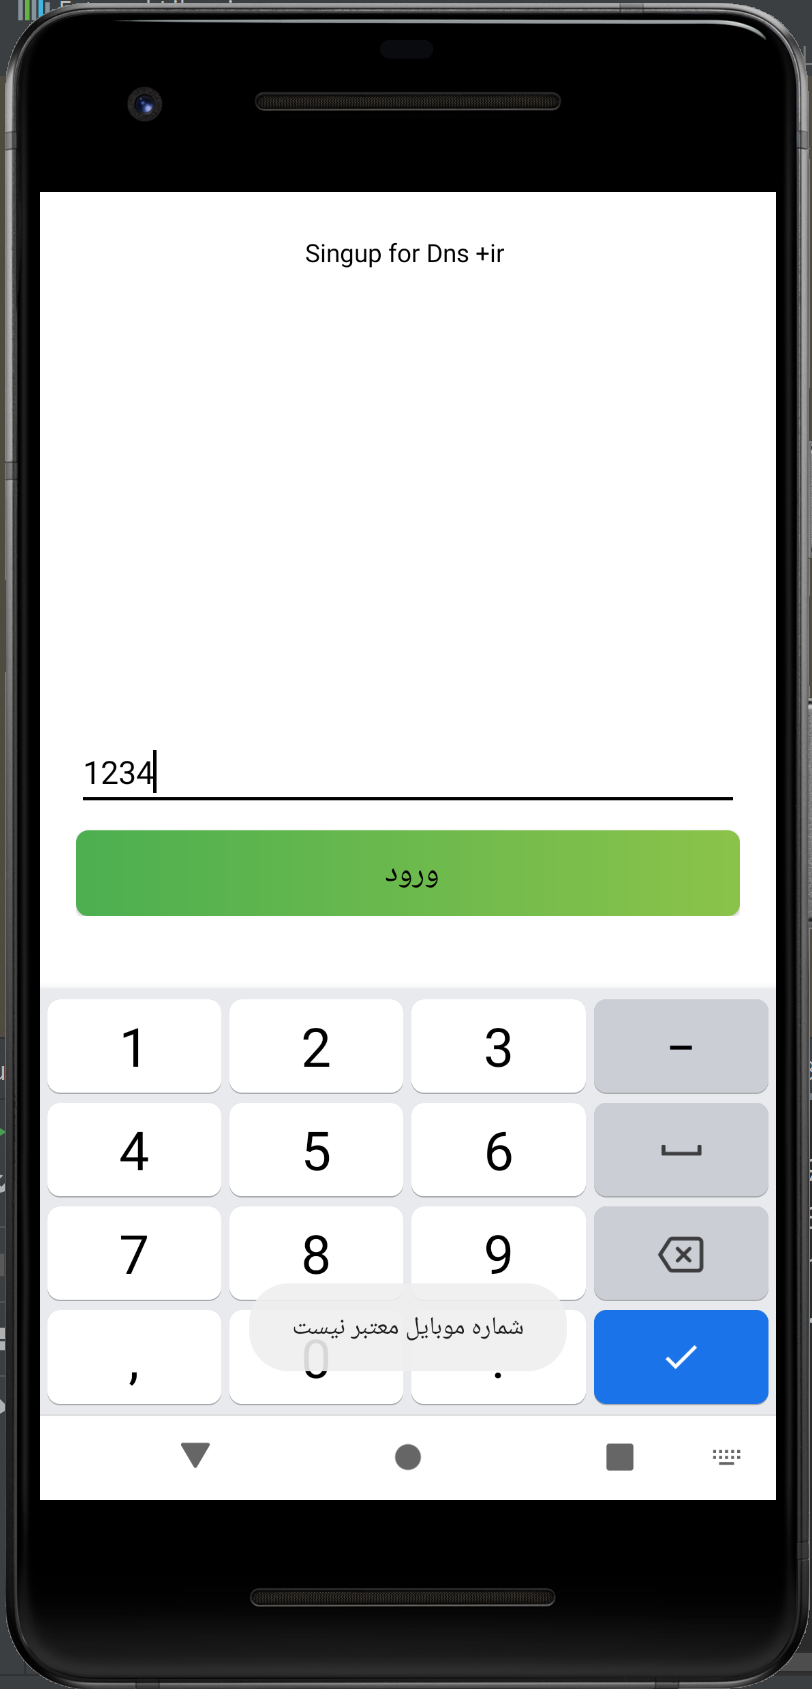
\includegraphics[width=1\textwidth]{./images/screenshot/SanaSystem/dynamic_and_proxy/wrong_number.png}
	    \caption{inserting a non-iranian number results in an error}
	    \label{fig:sana-system-wrong-number}
    \end{subfigure}
    \begin{subfigure}[h]{0.32\textwidth}
	    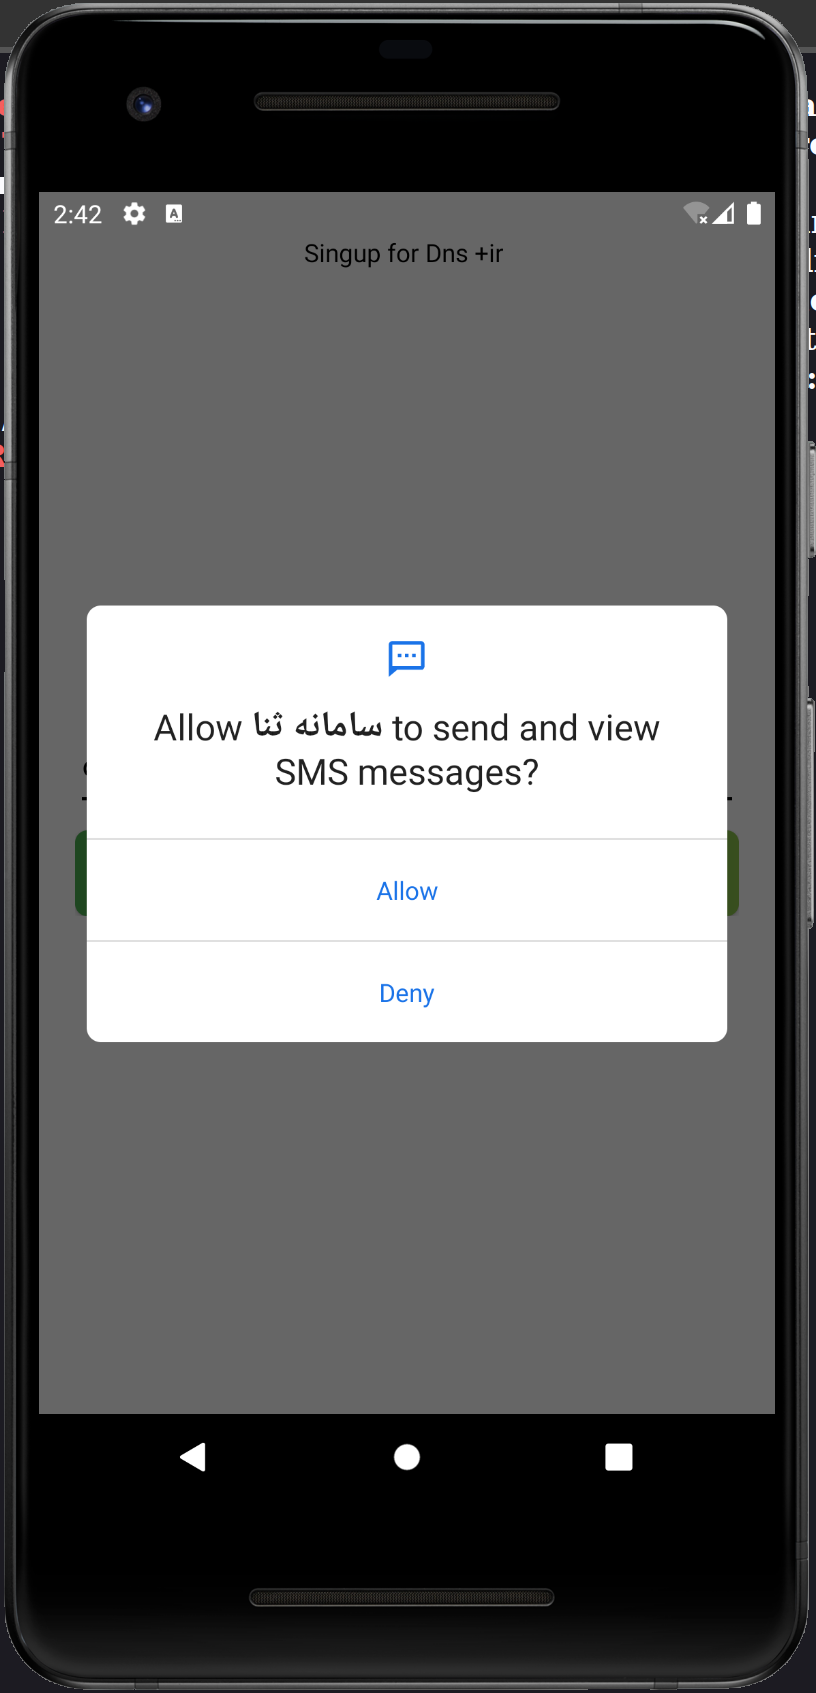
\includegraphics[width=1\textwidth]{./images/screenshot/SanaSystem/dynamic_and_proxy/correct_number_allow_sms.png}
	    \caption{request to access SMS messages}
	    \label{fig:sana-system-allow-sms}
    \end{subfigure}
    \caption{screenshots from Sana System's execution}
\end{figure}
After being launched, we get the input form built by the \texttt{MainActivity} class, shown in Fig. \ref{fig:sana-system-main-page}

Inserting a phone number not starting with an iranian prefix results in an error, shown by the pop-up toast message appearing at the bottom of Fig. \ref{fig:sana-system-wrong-number}

The first time that a correct number gets inserted, the application requests the permission to read and write SMS messages, as shown in Fig. \ref{fig:sana-system-allow-sms}. Denying it will take us back to the input form.

Allowing the SMS access permission, the application tries to load the phishing web page at the endpoint \texttt{/pishgiri} in an embedded WebView, where it presumably presses the victim to insert its credentials.

To see the actual packets sent to the server, we needed to install a custom certificate on the device, which allows a local proxy to intercept all the SSL encrypted traffic.
Because applications on Android aren't allowed by default to trust user specified certificates, we had to repackage and resign the apk, changing the trust anchors in the \texttt{res/xml/Network\_security\_config.xml} file.
Finally, given that the domain \texttt{https://eblaquie.org} doesn't exists anymore, the actual request might not even be made by the client; therefore we employed a custom DNS server on a local network to resolve the domain name to a local honeypot server.

With this setup, we were able to see all the traffic generated by the virus, using Burp Suite's (\url{https://portswigger.net/burp}) proxy feature.

\begin{figure}[h!]
	\begin{subfigure}[h]{\textwidth}
	    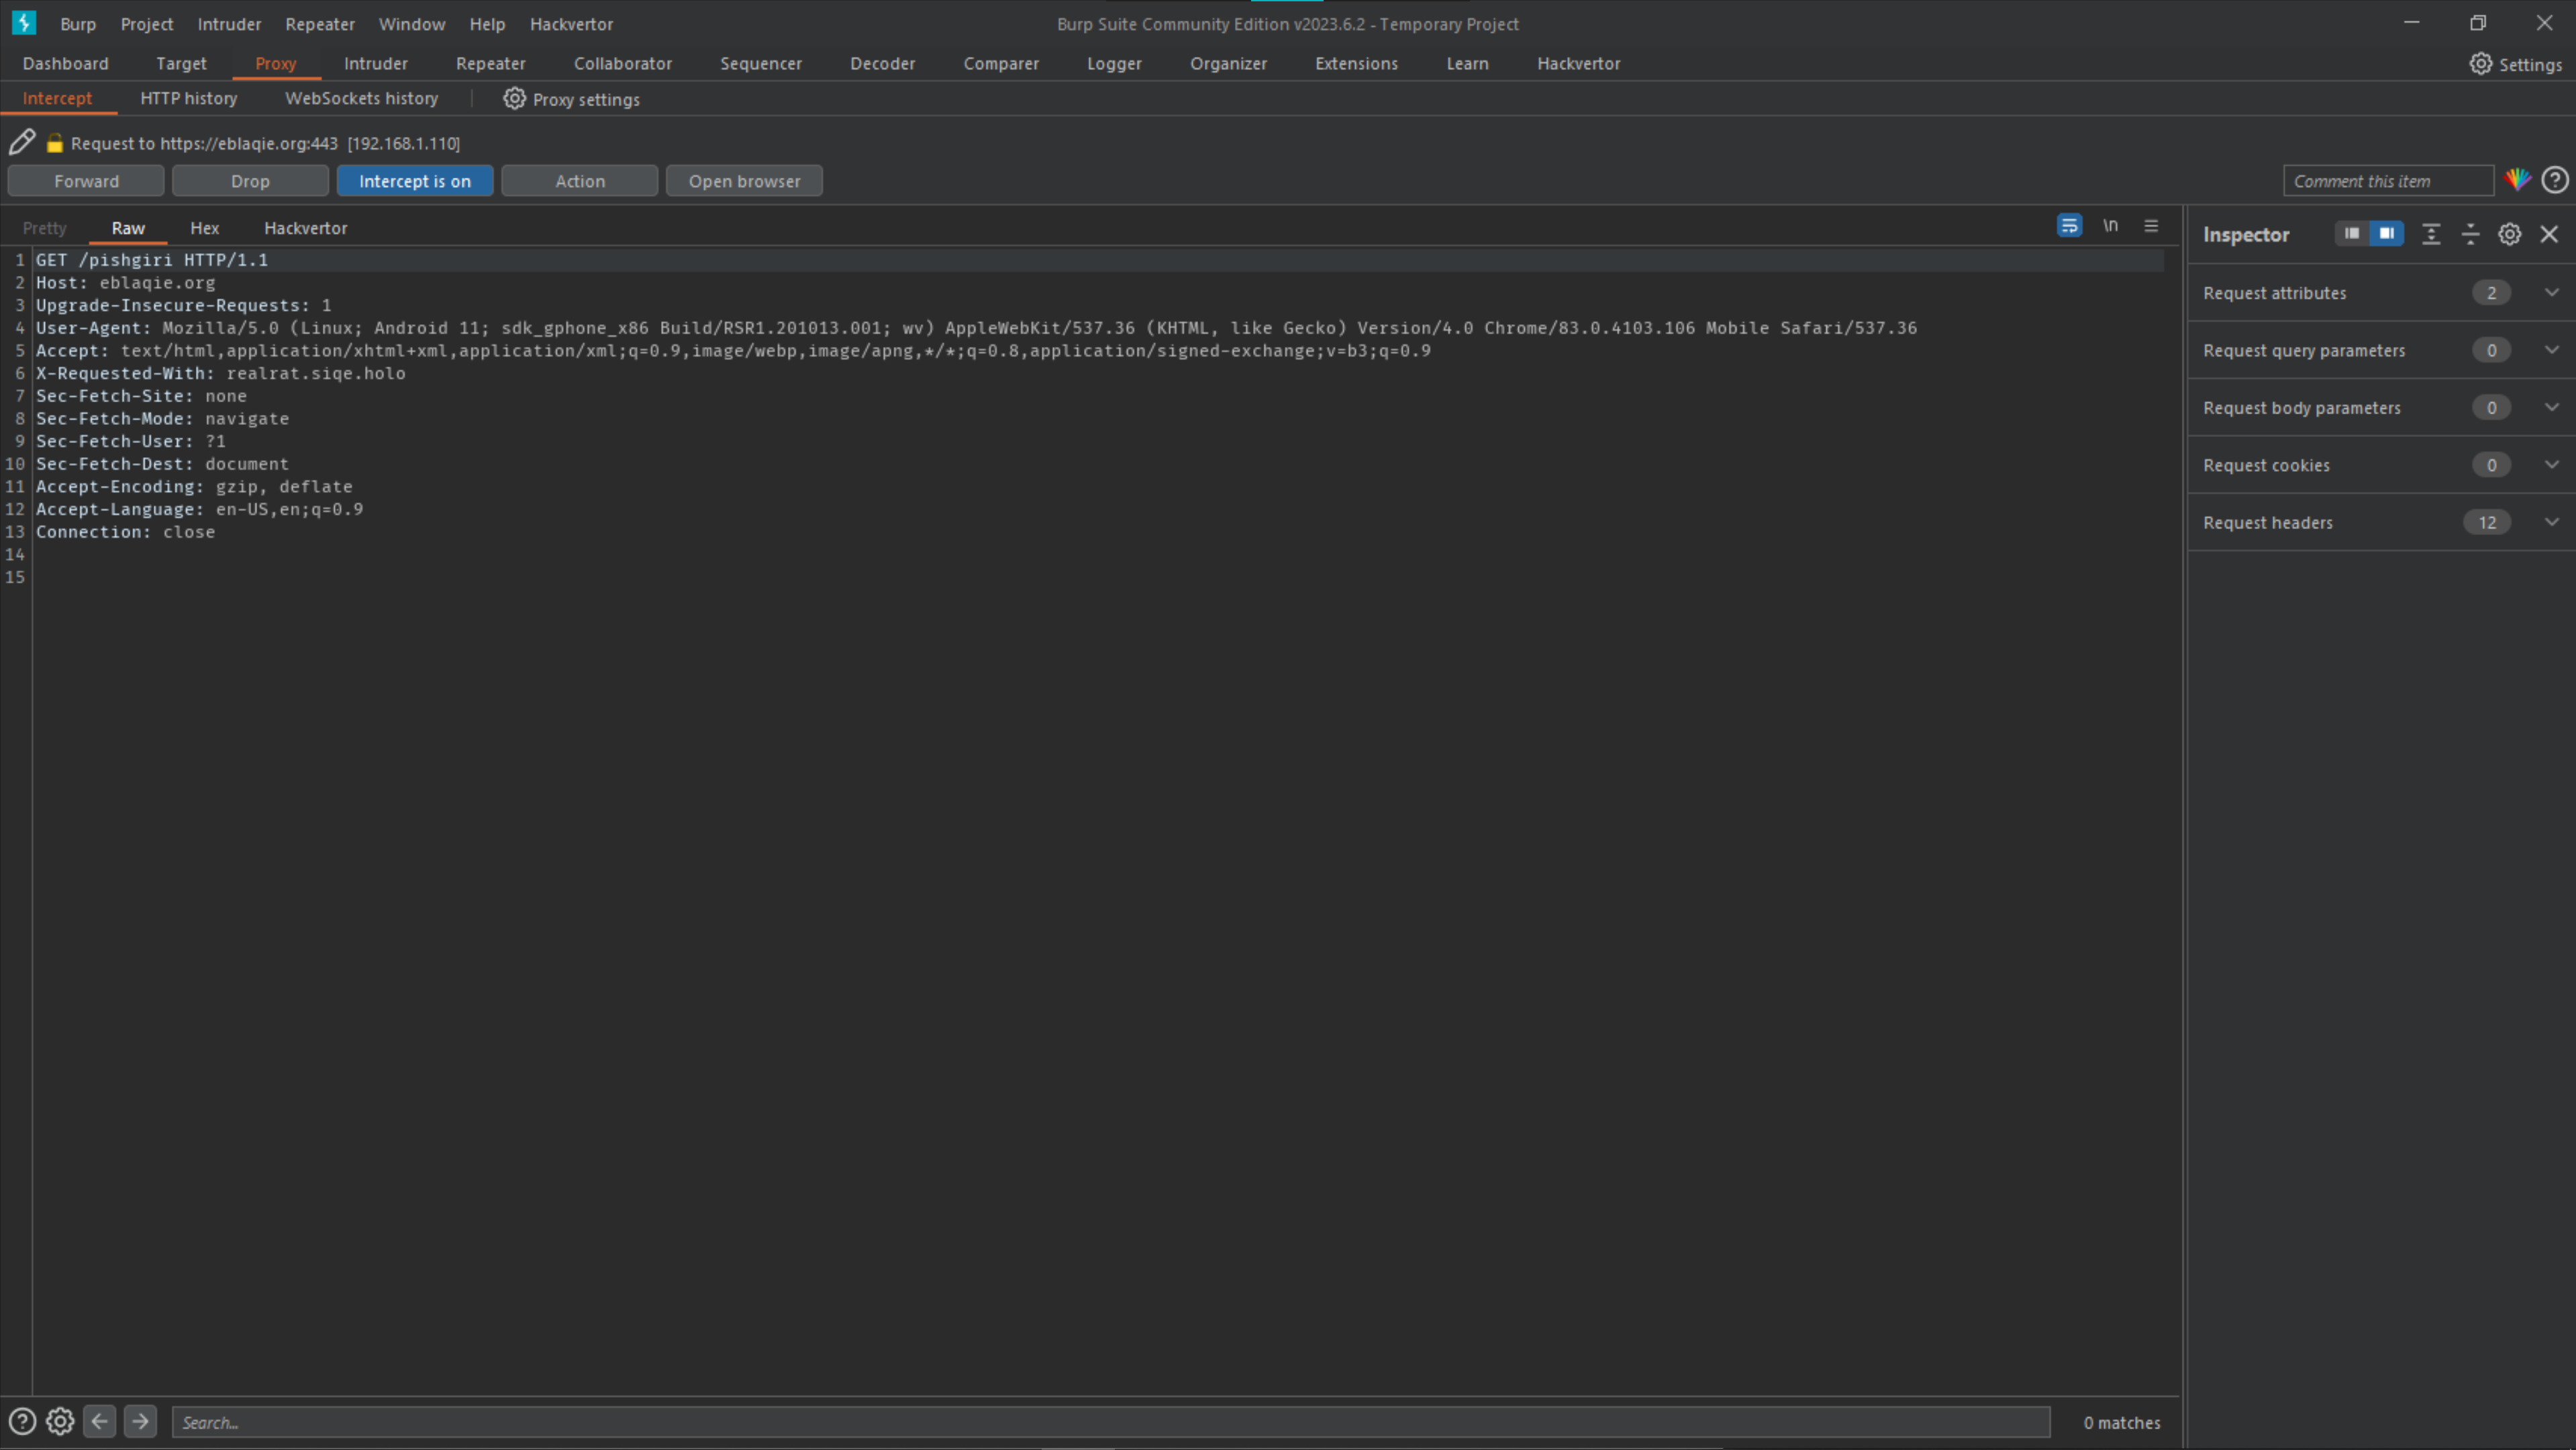
\includegraphics[width=1\textwidth]{./images/screenshot/SanaSystem/dynamic_and_proxy/phishing_site_connection.png}
	    \caption{connection to the phishing site}
	    \label{fig:sana-system-phishing-site-connection}
    \end{subfigure}
    \begin{subfigure}[h]{\textwidth}
	    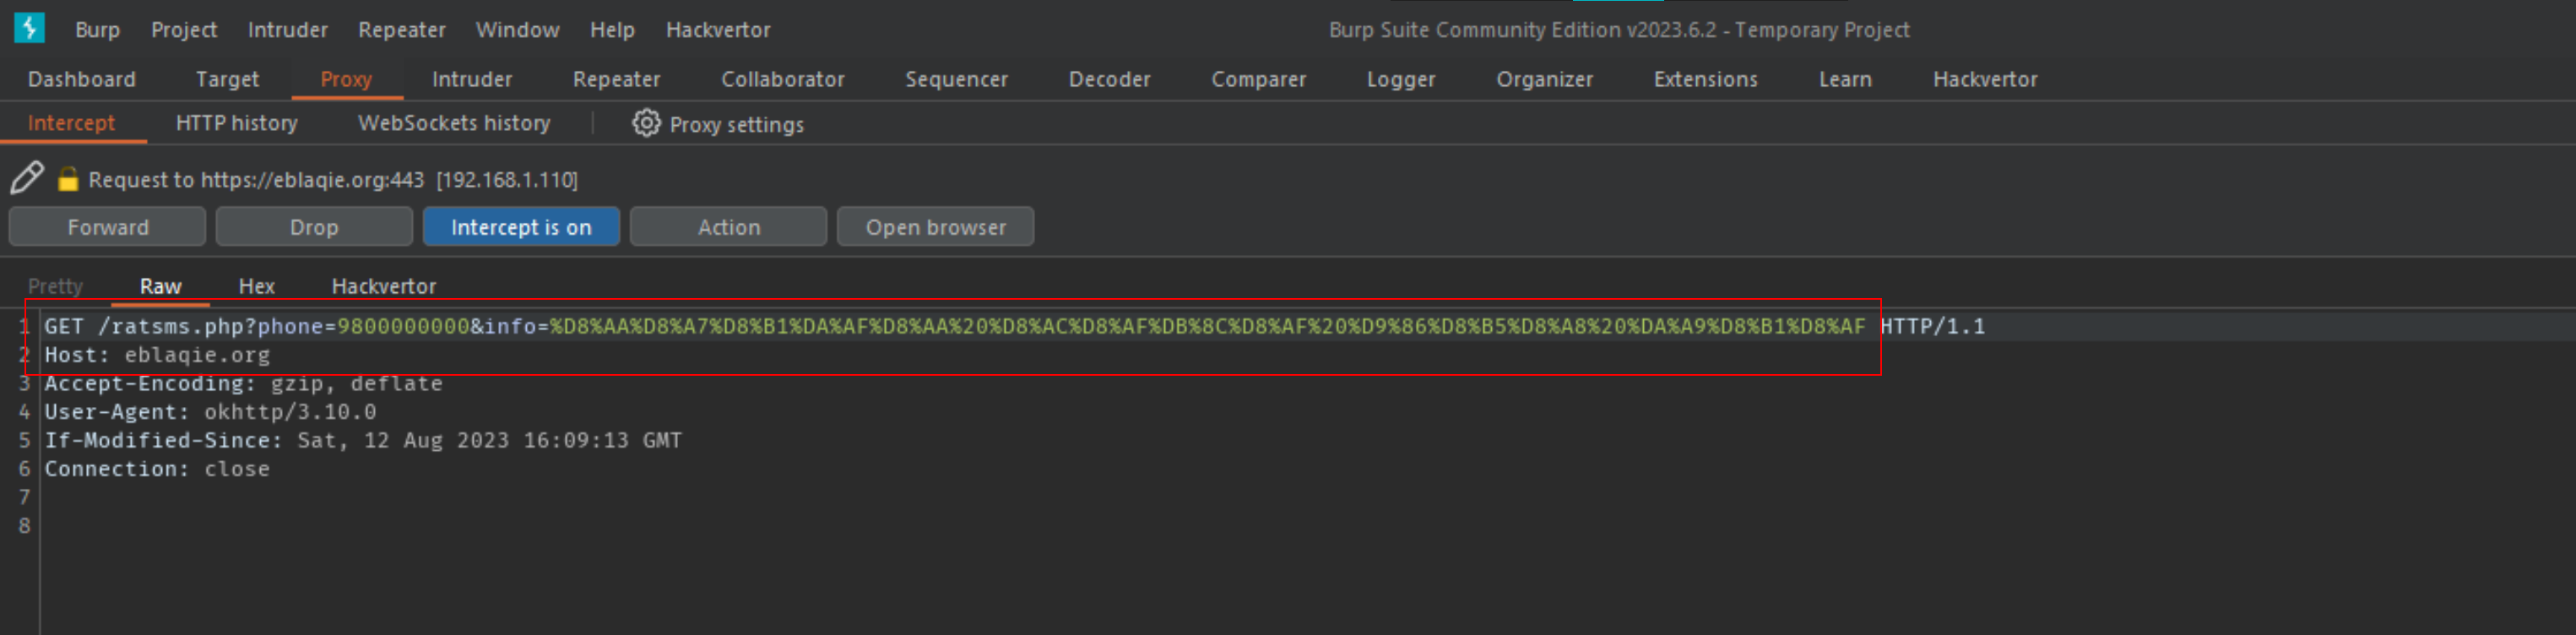
\includegraphics[width=1\textwidth]{./images/screenshot/SanaSystem/dynamic_and_proxy/first_connection.png}
	    \caption{first connection of a new number to the malicious server}
	    \label{fig:sana-system-first-connection}
    \end{subfigure}
    \begin{subfigure}[h]{\textwidth}
	    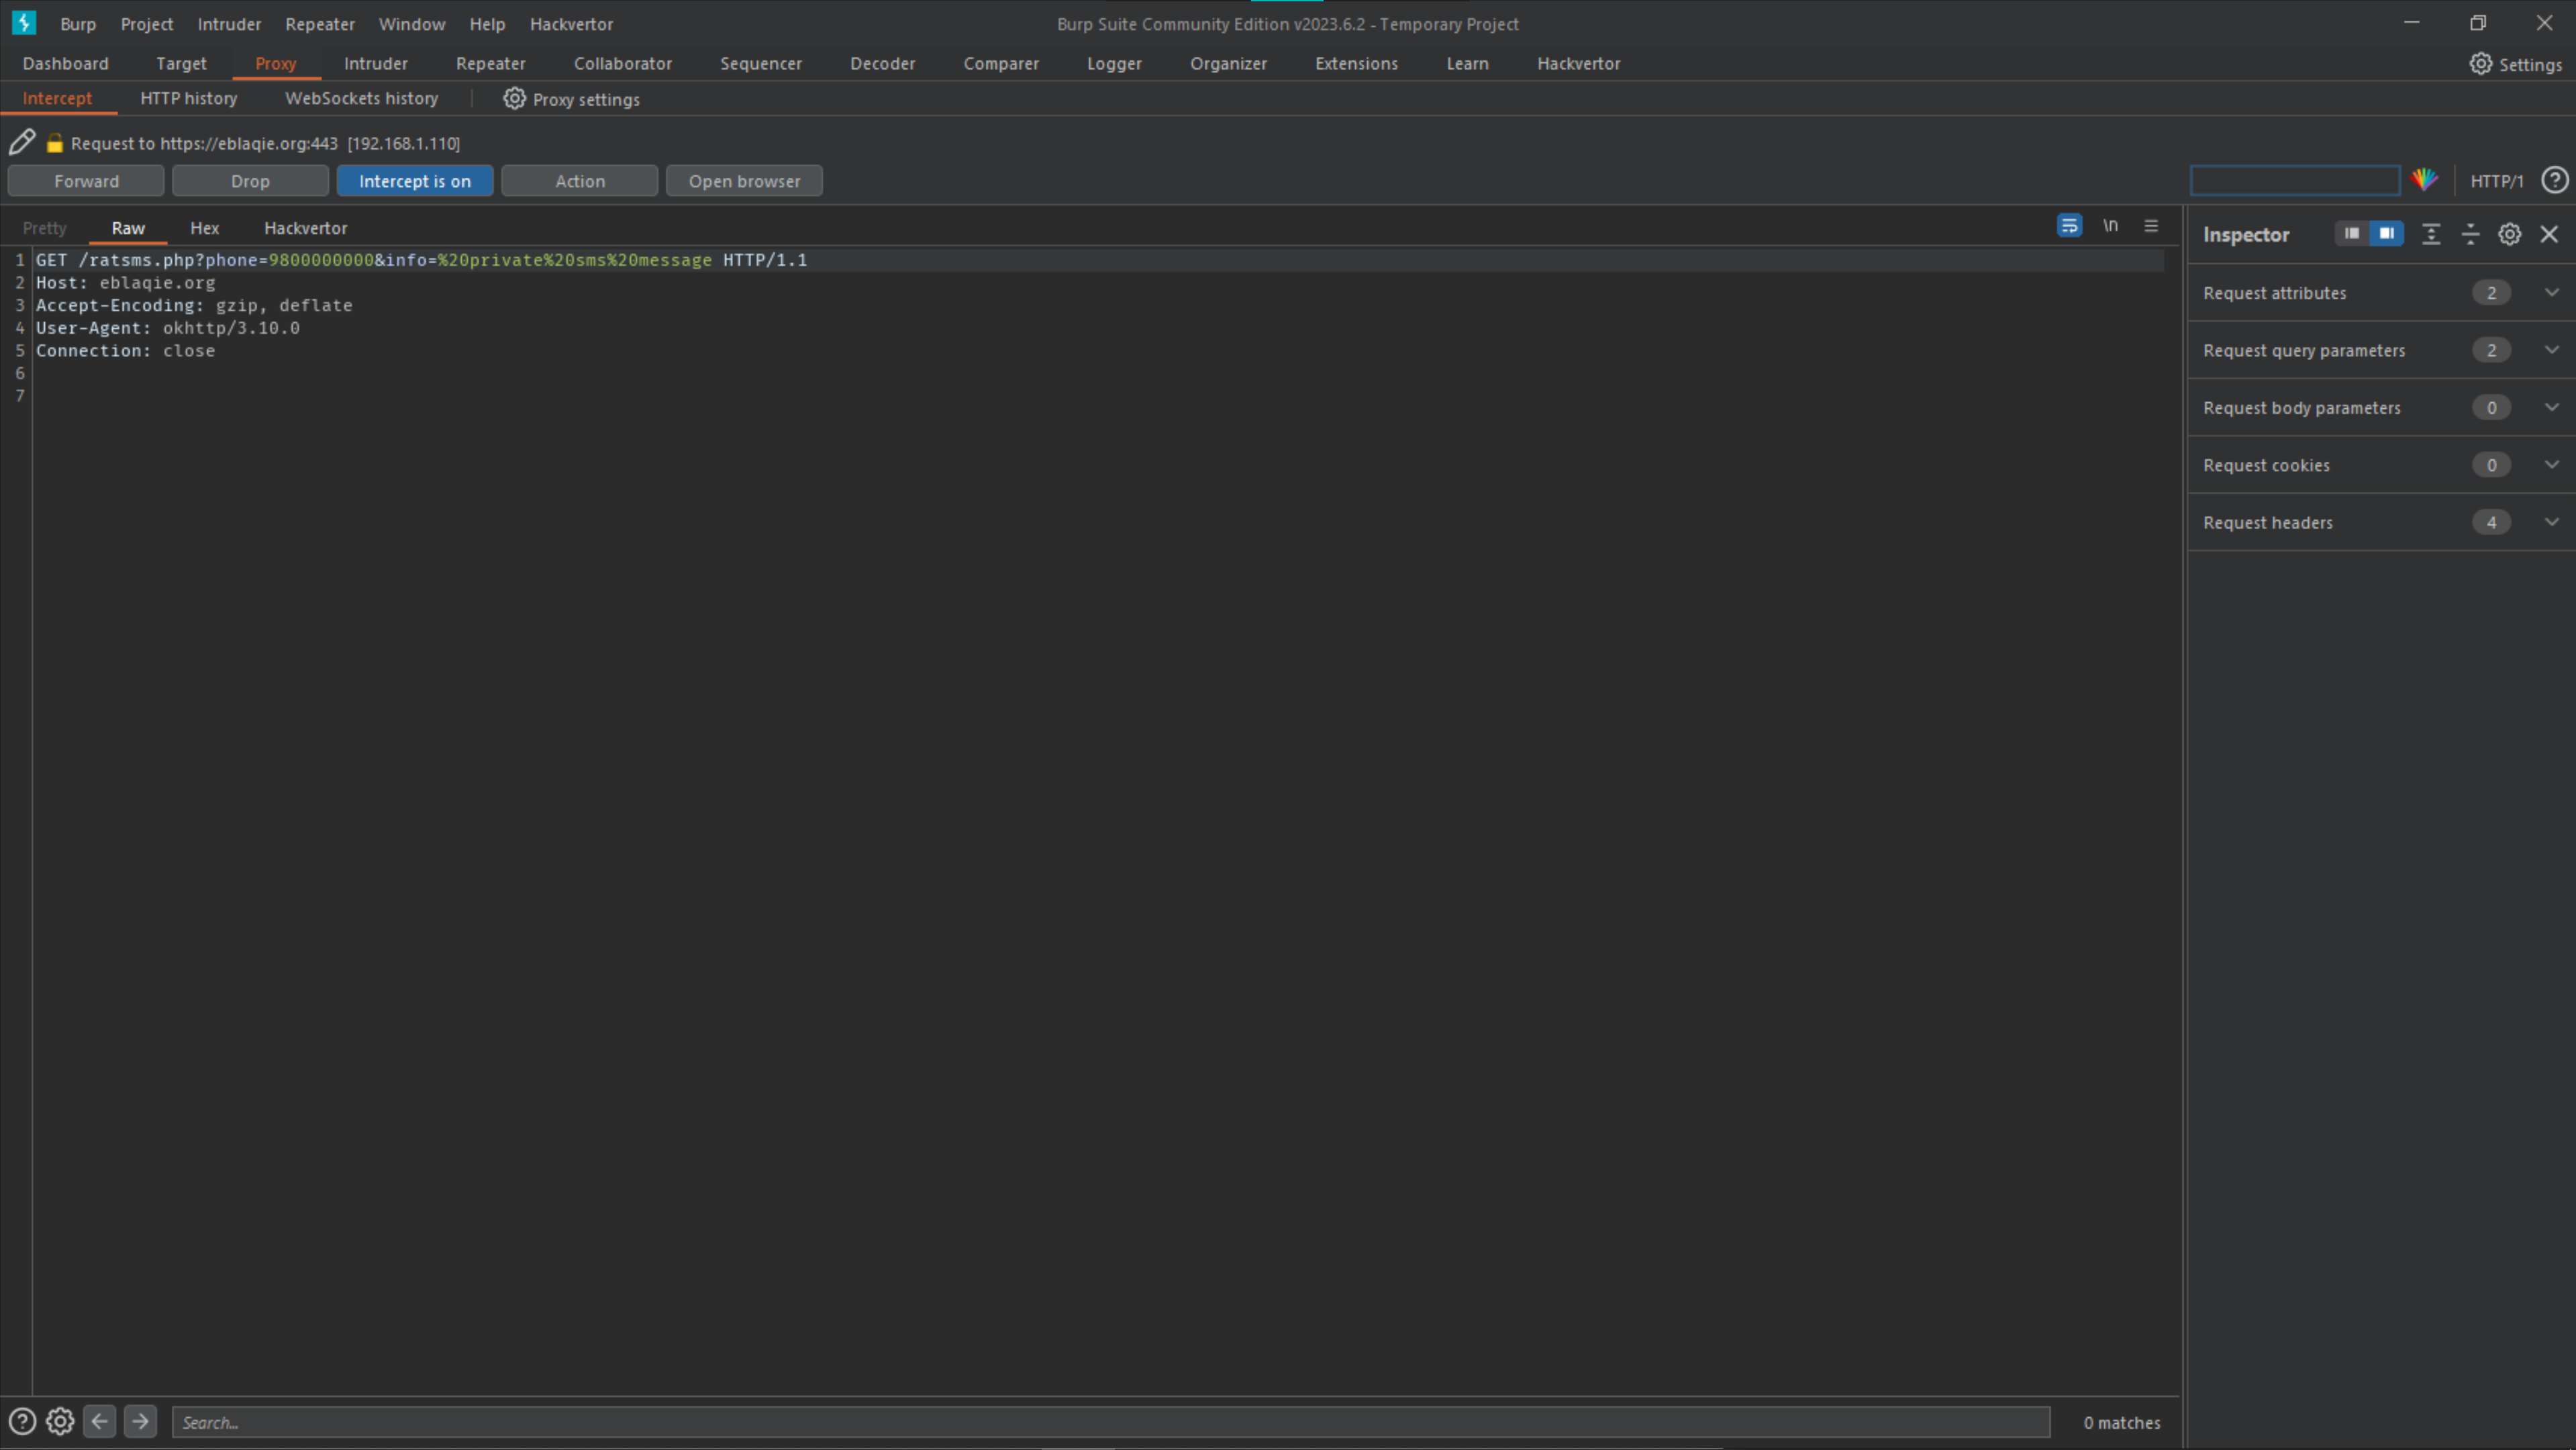
\includegraphics[width=1\textwidth]{./images/screenshot/SanaSystem/dynamic_and_proxy/sms_intercept_connection.png}
	    \caption{the content of each SMS received gets forwarded to the remote server}
	    \label{fig:sana-system-sms-intercept}
    \end{subfigure}
    \caption{screenshots from Sana System's execution}
\end{figure}

The connection to the phishing webpage is a simple GET request to the \texttt{/pishgiri} endpoint, as shown in Fig. \ref{fig:sana-system-phishing-site-connection}. We cannot be sure that more subpages existed under this fake website. When an iranian phone number gets correctly recognized by the input form, it gets immediately relayed to the \texttt{/ratsms.php} endpoint and tagged as a newly acquired target, as shown in Fig. \ref{fig:sana-system-first-connection}. Using the emulator's features, we were able to simulate the reception of an SMS message which, as we can see in Fig. \ref{fig:sana-system-sms-intercept}, gets immediately intercepted by the virus, and its content relayed to the same \texttt{/ratsms.php} endpoint. The text of the message (\textit{a private sms message}) can be read url-encoded in the \texttt{?info=} parameter.